% presentation
\documentclass[comptress]{beamer}


% handout
%\documentclass[handout,fleqn]{beamer}


% \mode<beamer>{
%   \usetheme{Madrid}
%   \mode<presentation>
% }

% \mode<handout>{
%   \usepackage{pgfpages}
%   \pgfpagesuselayout{2 on 1}[a4paper]
%   %\pgfpagesuselayout{4 on 1}[a4paper,landscape]
% }

\usepackage{mtex,fancyvrb,booktabs}
\usepackage{tikz}


\author[R. Hielscher, F. Bachmann]{Ralf Hielscher and Florian Bachmann}

\title[{\bf{\color{red}M}TEX} - an texture analysis
toolbox]{{\bf{\huge{\color{red}M}TEX}} \\ an open source texture analysis
toolbox}

\institute[Germany]{TU Chemnitz, TU Freiberg, Germany}


\date{Indianapolis, 2013}

\begin{document}

\frame[plain]{\titlepage}

%\begin{frame}

%  \tableofcontents

%\end{frame}


\section{What is MTEX?}
\label{sec:feature-overview}

\begin{frame}[fragile]
  \frametitle{What is MTEX?}

  \begin{overlayarea}{\textwidth}{3cm}
    \begin{enumerate}
      \item<1-> a MATLAB toolbox for quantitative texture analysis
      \item<2-> a scripting language
      \item<7-> a tool for generating publication ready plots
      \item<8-> large, well documented and exhaustively tested
      \item<9-> free to use, to extend, to modify
    \end{enumerate}
  \end{overlayarea}

  \bigskip

  \begin{overlayarea}{\textwidth}{5cm}
    \begin{onlyenv}<1>

      \centering{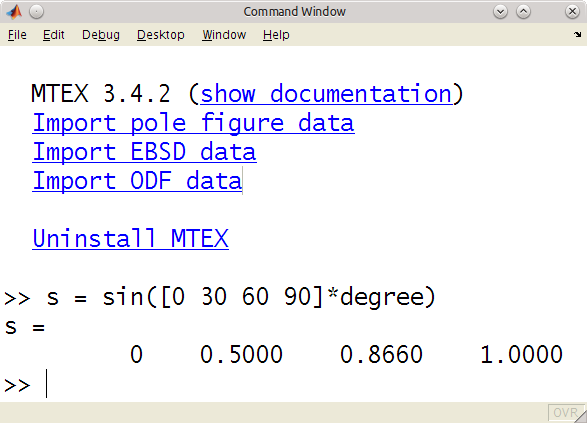
\includegraphics[height=5cm]{pic/snapshot1}}

    \end{onlyenv}


    \begin{onlyenv}<2>
      \begin{quote}
        why scripts?
        \begin{itemize}
          \item reproducible results
          \item templates for common tasks
          \item extensively customizable
          \item batch processing of many data sets
          \item repeated calculations with different parameters
        \end{itemize}
      \end{quote}

    \end{onlyenv}

    \begin{onlyenv}<3>
\begin{lstlisting}[style=input]
ebsd = loadEBSD('mylonite.txt') % load data

grains = calcGrains(ebsd)      % reconstruct grains

grainArea = area(grains)       % compute grain area

[m,index] = max(grainArea)     % find largest grain

plot(grains(index))            % plot largest grain
\end{lstlisting}
    \end{onlyenv}

    \begin{onlyenv}<4-6>
      \begin{lstlisting}[style=input]
ebsd = loadEBSD('mylonite.txt')
      \end{lstlisting}
    \end{onlyenv}
    \begin{onlyenv}<5-6>
      \vspace{-0.4cm}
      \begin{lstlisting}[style=input]
grains = calcGrains(ebsd)
    \end{lstlisting}
    \end{onlyenv}
    \begin{onlyenv}<6>
      \vspace{-0.4cm}
      \begin{lstlisting}[style=input]
grainArea = area(grains)
[m,index] = max(grainArea)
    \end{lstlisting}
    \end{onlyenv}
\begin{onlyenv}<4>
\begin{lstlisting}[style=output]
ebsd = /+EBSD+/ (show methods, plot)
  file name: mylonite.txt
  Properties: x, y
  Phase Orientations    Mineral Symmetry Crystal reference frame
      1         3444   Andesina       -1             X||a*, Z||c
      2         3893     Quartz      -3m      X||a*, Y||b,  Z||c*
      3          368    Biotite      2/m      X||a*, Y||b*, Z||c
      4         4781 Orthoclase      2/m      X||a*, Y||b*, Z||c
  \end{lstlisting}
    \end{onlyenv}
\begin{onlyenv}<5>
\begin{lstlisting}[style=output]
grains = /+Grain2d-Set+/ (show methods, plot)
  file name: mylonite.txt
  EBSD properties: x, y, mis2mean
  Phase Grains Orient.    Mineral Symmetry Cryst. reference frame
      1   1951    3444   Andesina       -1          X||a*, Z||c
      2    776    3893     Quartz      -3m   X||a*, Y||b,  Z||c*
      3    305     368    Biotite      2/m   X||a*, Y||b*, Z||c
      4   1641    4781 Orthoclase      2/m   X||a*, Y||b*, Z||c
  \end{lstlisting}
\end{onlyenv}
\begin{onlyenv}<6>
\begin{lstlisting}[style=output]
m =
   1.4985e+06
index =
        1795
\end{lstlisting}
\end{onlyenv}
%     \begin{onlyenv}<2-3>
%    \begin{lstlisting}[style=input]
% h = Miller(1,-2,1,0,symmetry('quartz'))
%    \end{lstlisting}
% \end{onlyenv}
% \begin{onlyenv}<2>
% \begin{lstlisting}[style=output]
% h = /+Miller+/ (show methods, plot)
%   size: 1 x 1
%   mineral: Quartz (P 32 2 1, X||a*, Y||b, Z||c*)
%   h  1
%   k -2
%   i  1
%   l  0
% \end{lstlisting}
% \end{onlyenv}
%    \begin{onlyenv}<3>
%      \vspace{-0.3cm}
%   \begin{lstlisting}[style=input]
% a = angle(h,xvector) / degree
%   \end{lstlisting}
% \begin{lstlisting}[style=output]
% a =
%    30.0000
% \end{lstlisting}
% \end{onlyenv}

\begin{onlyenv}<8>
  \begin{quote}
  \begin{itemize}
    \item 6 years of development
    \item 1000 functions
    \item 40 000 lines of code, 33 percent comment lines
    \item 14 reference paper, about 200 references
    \item 300 to 1000 downloads per version
    \item 1000 help pages
    \item compatible toolboxes: MSAT, PolyLx
  \end{itemize}
  \end{quote}
\end{onlyenv}


\begin{onlyenv}<7>
  \centerline{
  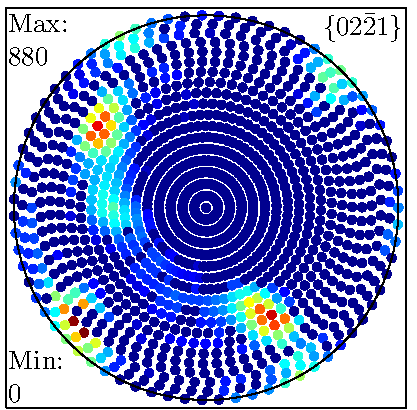
\includegraphics[height=4cm]{pic/pf1}
  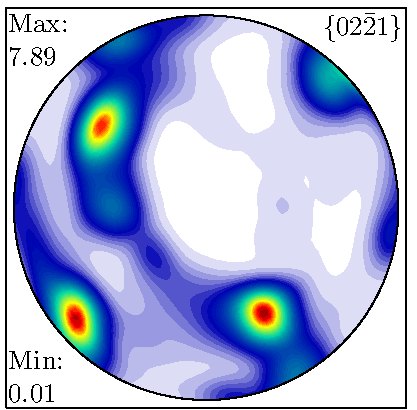
\includegraphics[height=4cm]{pic/pdf1}
  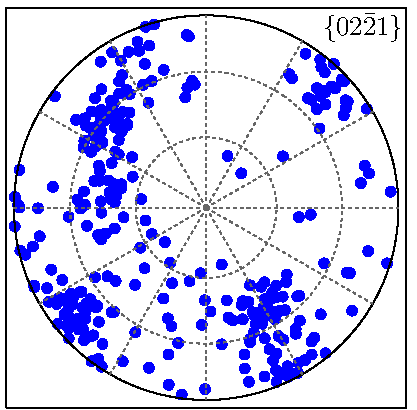
\includegraphics[height=4cm]{pic/ebsd1}
  }
\end{onlyenv}

\begin{onlyenv}<9>
  \centerline{
  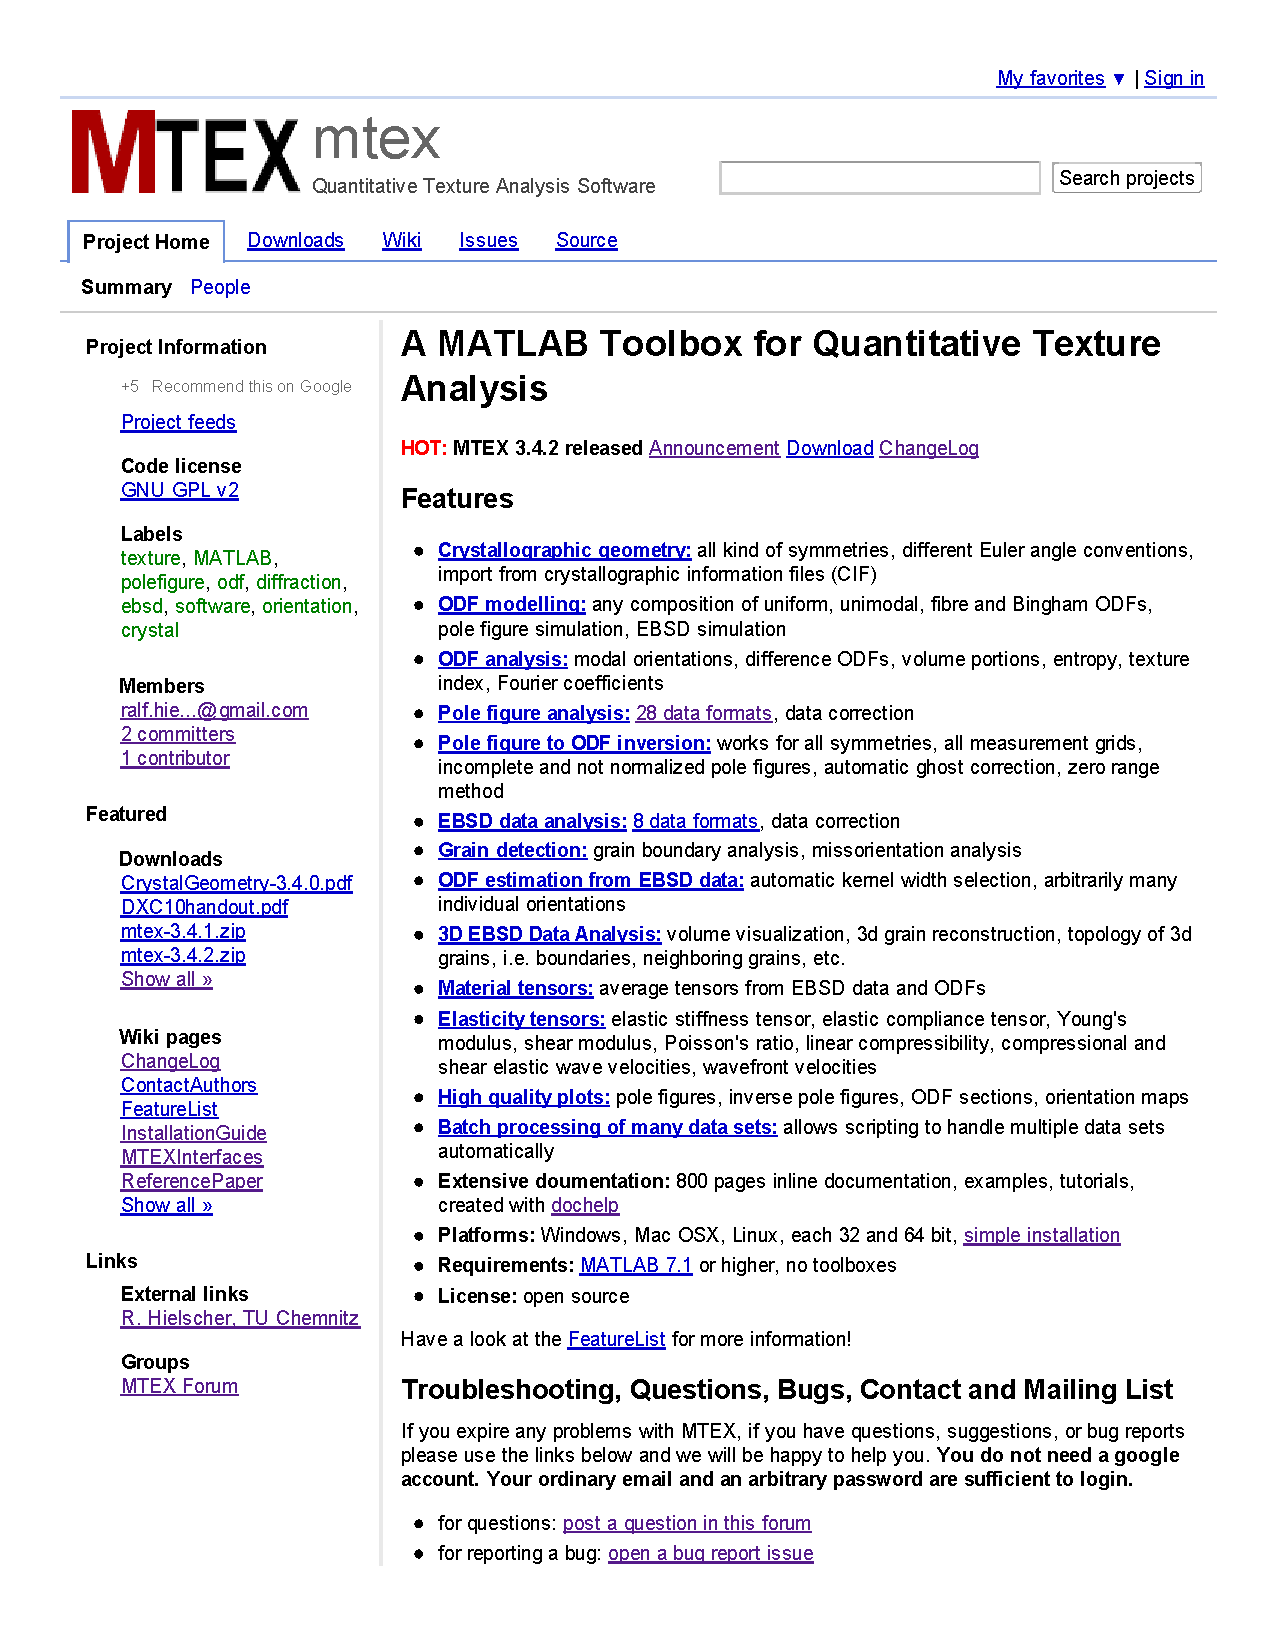
\includegraphics[width=\textwidth]{pic/mtex}
  }
\end{onlyenv}

\end{overlayarea}

\end{frame}


\section{A Feature Overview}

\begin{frame}[fragile]
  \frametitle{Feature Overview}

  \begin{overlayarea}{\textwidth}{2.5cm}
    \begin{itemize}
      \item<1-> crystal geometry
      \item<4-> odf modeling
      \item<5-> pole figure measurements
      \item<9-> individual orientation measurements
      \item<13-> elastic and plastic deformations
  \end{itemize}
  \end{overlayarea}

  \bigskip

  \begin{overlayarea}{\textwidth}{5.5cm}

  \begin{onlyenv}<1-2>
      \begin{lstlisting}[style=input]
ori1 = orientation('Euler',10*degree,20*degree,0,...
       symmetry('quartz'))
  \end{lstlisting}
\end{onlyenv}
  \begin{onlyenv}<1>
\begin{lstlisting}[style=output]
ori1 = /+orientation+/ (show methods, plot)
  size: 1 x 1
  crystal symmetry: Quartz (P 32 2 1, X||a*, Y||b, Z||c*)
  sample symmetry : triclinic

  Bunge Euler angles in degree
  phi1  Phi phi2
    10   20    0
  \end{lstlisting}
  \end{onlyenv}
  \begin{onlyenv}<2>
    \vspace{-0.3cm}
    \begin{lstlisting}[style=input]
r = ori1 * Miller(1,1,-2,0,symmetry('quartz'))
    \end{lstlisting}
    \begin{lstlisting}[style=output]
r = /+vector3d+/ (show methods, plot)
  size: 1 x 1
         x        y        z
  0.305126 0.176165 0.203417
    \end{lstlisting}
  \end{onlyenv}
  \begin{onlyenv}<3>
      \begin{lstlisting}[style=input]
ori2 = orientation('Euler',50*degree,0,20*degree,...
       symmetry('olivin'))
mori = inv(ori1) * ori2
  \end{lstlisting}
  \begin{lstlisting}[style=output]
mori = /+misorientation+/ (show methods, plot)
  size: 1 x 1
  crystal symmetry: IRON TETRATHIOSILICATE (P n m a)
  crystal symmetry: Quartz (P 32 2 1, X||a*, Y||b, Z||c*)

  Bunge Euler angles in degree
  phi1  Phi phi2
    60   90   40
  \end{lstlisting}
  \end{onlyenv}
  \begin{onlyenv}<4>
    \begin{lstlisting}[style=input]
odf = 0.8 * unimodalODF(ori1) + ...
      0.2 * uniformODF(symmetry('quartz'))
  \end{lstlisting}
  \vspace{-0.2cm}
  \begin{lstlisting}[style=output]
odf = /+ODF+/ (show methods, plot)
  crystal symmetry: Quartz (P 32 2 1, X||a*, Y||b, Z||c*)
  sample symmetry : triclinic

  Radially symmetric portion:
    kernel: de la Vallee Poussin, hw = 10°
    center: (30°,90°,0°)
    weight: 0.8

  Uniform portion:
    weight: 0.2
  \end{lstlisting}
\end{onlyenv}

\begin{onlyenv}<5-6>
  \begin{lstlisting}[style=input]
pf = loadPoleFigure('Queens_alu.plf')
  \end{lstlisting}
\end{onlyenv}
\begin{onlyenv}<6>
  \vspace{-0.3cm}
  \begin{lstlisting}[style=input]
plot(pf)
  \end{lstlisting}
\end{onlyenv}
\begin{onlyenv}<5>
\begin{lstlisting}[style=output]
pf = /+PoleFigure+/ (show methods, plot)
  file name: Queens_alu.plf
  crystal symmetry : cubic (m-3m)
  specimen symmetry: orthorhombic

  h = {111}, r = 90x17 points
  h = {200}, r = 90x17 points
  h = {220}, r = 90x17 points
  h = {311}, r = 90x17 points
  \end{lstlisting}
\end{onlyenv}
\begin{onlyenv}<6>
  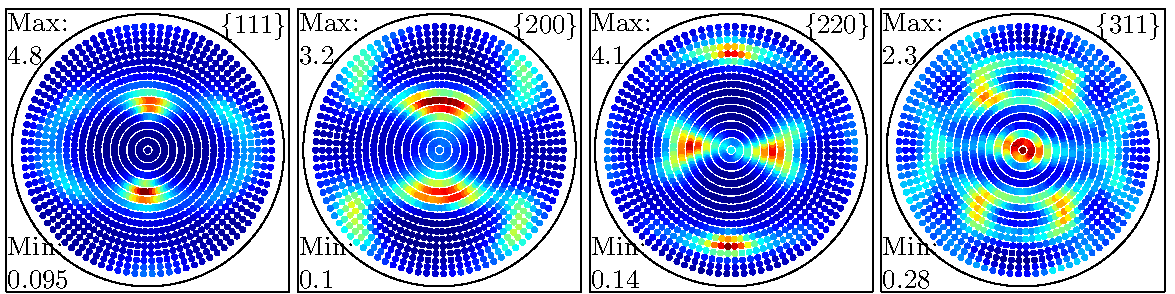
\includegraphics[width=\textwidth]{pic/pf}
\end{onlyenv}
\begin{onlyenv}<7-8>
  \begin{lstlisting}[style=input]
odf = calcODF(pf)
  \end{lstlisting}
\end{onlyenv}
\begin{onlyenv}<8>
  \vspace{-0.3cm}
  \begin{lstlisting}[style=input]
plotpdf(odf,get(pf,'h'))
  \end{lstlisting}
\end{onlyenv}
\begin{onlyenv}<7>
\begin{lstlisting}[style=output]
odf = /+ODF+/ (show methods, plot)
  file name: Queens_alu.plf
  crystal symmetry: cubic
  sample symmetry : orthorhombic

  Uniform portion:
    weight: 0.14633

  Radially symmetric portion:
    kernel: de la Vallee Poussin, hw = 4°
    center: 2444 orientations, resolution: 3.9°
    weight: 0.85367
  \end{lstlisting}
\end{onlyenv}
\begin{onlyenv}<8>
  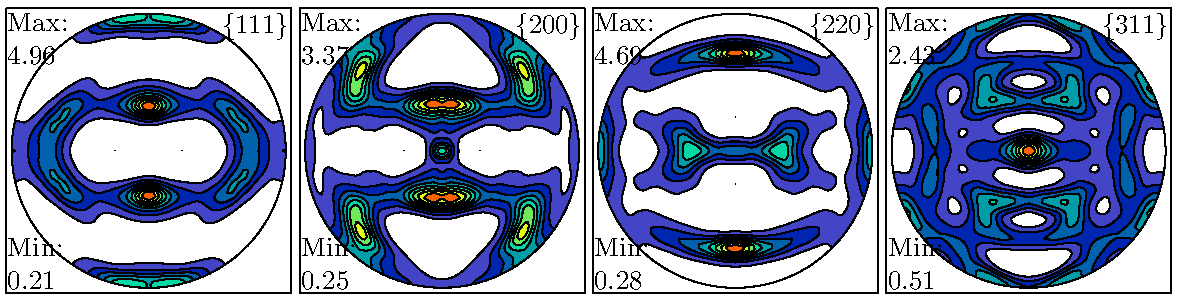
\includegraphics[width=\textwidth]{pic/pdf}
\end{onlyenv}
\begin{onlyenv}<9-10>
  \begin{lstlisting}[style=input]
ebsd = loadEBSD('mylonite.txt')
  \end{lstlisting}
\end{onlyenv}
\begin{onlyenv}<10>
  \vspace{-0.3cm}
  \begin{lstlisting}[style=input]
plot(ebsd)
  \end{lstlisting}
\end{onlyenv}
\begin{onlyenv}<9>
  \begin{lstlisting}[style=output]
ebsd = /+EBSD+/ (show methods, plot)
  file name: mylonite.txt
  Properties: x, y
  Phase Orientations    Mineral Symmetry Crystal reference frame
      1         3444   Andesina       -1             X||a*, Z||c
      2         3893     Quartz      -3m      X||a*, Y||b,  Z||c*
      3          368    Biotite      2/m      X||a*, Y||b*, Z||c
      4         4781 Orthoclase      2/m      X||a*, Y||b*, Z||c
  \end{lstlisting}
\end{onlyenv}
\begin{onlyenv}<10>
  \vspace{-0.75cm}
  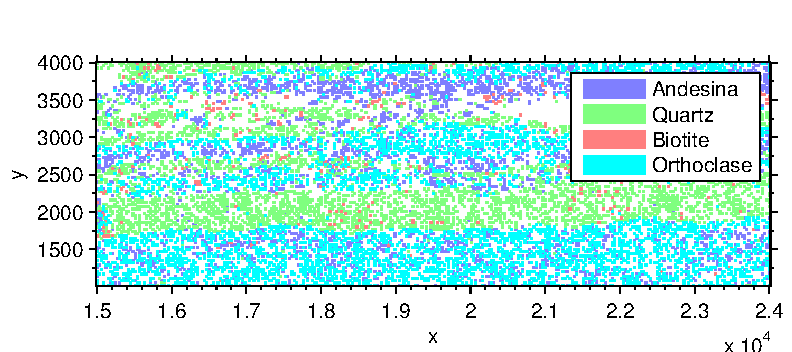
\includegraphics[width=0.9\textwidth]{pic/ebsdmylonite}
\end{onlyenv}
\begin{onlyenv}<11-12>
  \begin{lstlisting}[style=input]
grains = calcGrains(ebsd)
  \end{lstlisting}
\end{onlyenv}
\begin{onlyenv}<12>
  \vspace{-0.4cm}
  \begin{lstlisting}[style=input]
plot(grains)
  \end{lstlisting}
\end{onlyenv}
\begin{onlyenv}<11>
  \begin{lstlisting}[style=output]
grains = /+Grain2d-Set+/ (show methods, plot)
  file name: mylonite.txt
  EBSD properties: x, y, mis2mean
  Phase Grains Orient.    Mineral Symmetry Cryst. reference frame
      1   1951    3444   Andesina       -1          X||a*, Z||c
      2    776    3893     Quartz      -3m   X||a*, Y||b,  Z||c*
      3    305     368    Biotite      2/m   X||a*, Y||b*, Z||c
      4   1641    4781 Orthoclase      2/m   X||a*, Y||b*, Z||c
  \end{lstlisting}
\end{onlyenv}
\begin{onlyenv}<12>
  \centerline{
  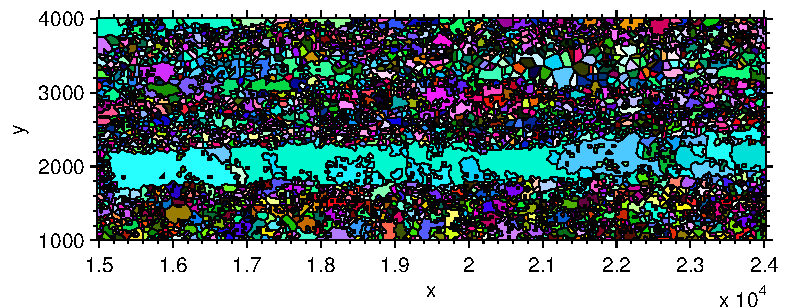
\includegraphics[width=0.9\textwidth]{pic/grainsMylonite}
  }
\end{onlyenv}
\begin{onlyenv}<13>
  \begin{lstlisting}[style=input]
cs = symmetry('Olivin');
C  = loadTensor('Olivine1997PC.GPa',cs,...
    'propertyname','elastic stiffness','unit','Pa')
  \end{lstlisting}
  \vspace{-.3cm}
  \begin{lstlisting}[style=output]
C = elastic stiffness /+tensor+/
  unit        : Pa
  mineral     : Olivin (mmm)

 320.5  68.2  71.6     0     0     0
  68.2 196.5  76.8     0     0     0
  71.6  76.8 233.5     0     0     0
     0     0     0    64     0     0
     0     0     0     0    77     0
     0     0     0     0     0  78.7
    \end{lstlisting}
\end{onlyenv}
\begin{onlyenv}<14>
  \begin{lstlisting}[style=input]
plot(C,'PlotType','velocity','vp','density')
plot(C,'PlotType','velocity','pp','density')
  \end{lstlisting}
  \centerline{
  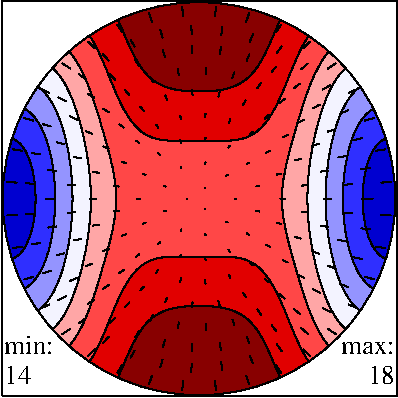
\includegraphics[height=3.5cm]{pic/vp-pp}
  \quad
  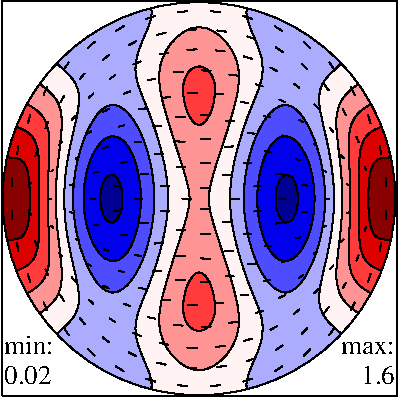
\includegraphics[height=3.5cm]{pic/vs12-ps1}
  \quad
  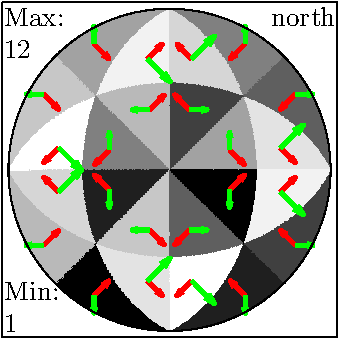
\includegraphics[height=3.5cm]{pic/activeSlip}
  }
\end{onlyenv}


\end{overlayarea}




\end{frame}


% \begin{frame}
%   \frametitle{Electron back scatter diffraction}

%   \begin{itemize}
%     \item reads 13 different file formats
%     \item data correction
%     \item grain segmentation
%     \item grain boundary analysis
%     \item misorientations analysis
%     \item ODF calculation
%   \end{itemize}
% \end{frame}

% \begin{frame}
%   \frametitle{Orientation distribution function}

%   \begin{itemize}
%     \item ODF modeling
%     \item pole figure calculation
%     \item individual orientation simulation
%     \item volume, fibre volume, modal orientation
%     \item ODF comparison
%     \item texture index, entropy
%     \item mean tensor
%     \item misorientation distribution function
%   \end{itemize}

% \end{frame}

% \begin{frame}
%   \frametitle{Pole Figure Data}

%   \begin{itemize}
%     \item import from 30 file formats
%     \item data correction
%     \item ODF reconstruction
%     \item automatic ghost correction
%     \item zero range method
%     \item arbitrary grids
%   \end{itemize}

% \end{frame}


% \begin{frame}
%   \frametitle{Elastic and Plastic Deformation}

%   \begin{itemize}
%     \item stress and strain tensors
%     \item Young's modulus
%     \item Christoffel tensor
%     \item piezo electricity
%     \item wave velocities
%     \item average tensors
%     \item Schmid tensor
%     \item active slips system
%   \end{itemize}
% \end{frame}


\begin{frame}[fragile]
  \frametitle{Benefits / Challenges of Big Projects}

  \begin{overlayarea}{\textwidth}{2.5cm}
  \begin{itemize}
    \item<2-> everything (needs to) works with everything
    \item<4-> less code duplication - bugs have greater impact
    \item<5-> additional features are simple / difficult to include
    \item<6-> you can (must) plot everything with the same engine
  \end{itemize}
\end{overlayarea}
\begin{overlayarea}{\textwidth}{5.5cm}
  \begin{onlyenv}<2>
    \begin{lstlisting}
density = calcAngleDistribution(ebsd)
density = calcAngleDistribution(grains)
density = calcAngleDistribution(sym)
density = calcAngleDistribution(mdf)
    \end{lstlisting}
  \end{onlyenv}
  \begin{onlyenv}<3>
    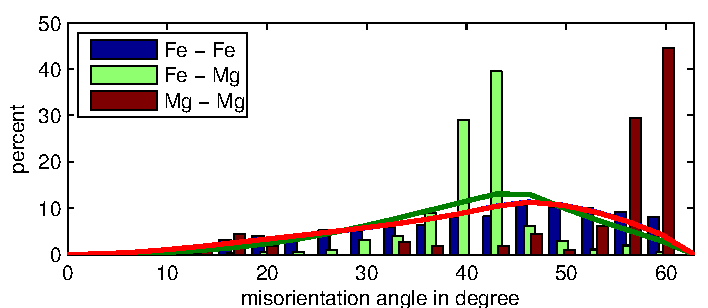
\includegraphics[width=\textwidth]{pic/misori}
  \end{onlyenv}
  \begin{onlyenv}<6>
    \vspace{-0.3cm}
  \begin{lstlisting}[sytle=input]
plot(pf)
plotpdf(odf,Miller(0,2,-2,1))
plotpdf(ebsd,Miller(0,2,-2,1))
  \end{lstlisting}

  \centerline{
  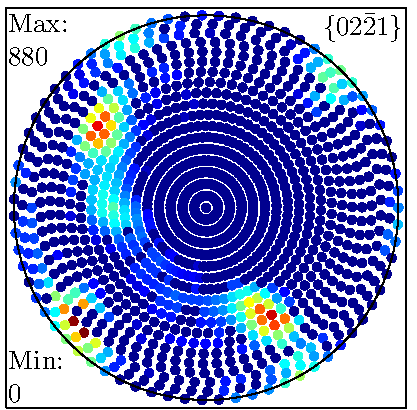
\includegraphics[height=3.5cm]{pic/pf1}
  \quad
  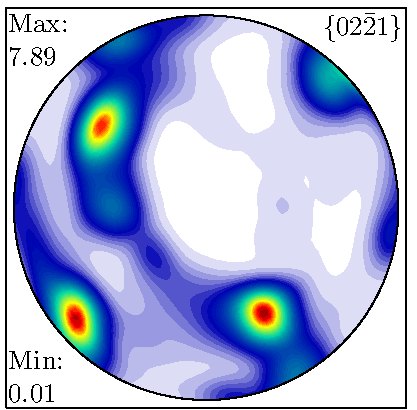
\includegraphics[height=3.5cm]{pic/pdf1}
  \quad
  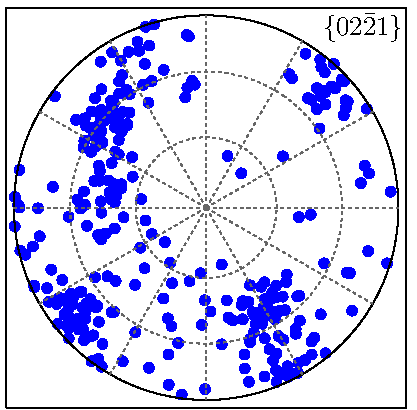
\includegraphics[height=3.5cm]{pic/ebsd1}
  }
\end{onlyenv}

\begin{onlyenv}<4-5>
  % \begin{quote}
  %   \begin{itemize}
  %     \item make functions as
  %   \end{itemize}
  % \end{quote}
  \vspace{-0.3cm}
      \begin{lstlisting}[type=input]
function nu = PoissonRatio(C,x,y)
% compute Poisson ration transverse x and axial y

S = inv(C); % compute the complience

% compute lateral and longitudinal strain
a = EinsteinSum(S,[-1 -2 -3 -4],x,-1,x,-2,y,-3,y,-4)
b = EinsteinSum(S,[-1 -2 -3 -4],x,-1,x,-2,x,-3,x,-4)

% negative quotient
nu = -double(a) ./  double(b);
    \end{lstlisting}
\end{onlyenv}

\end{overlayarea}

\end{frame}

\section{Design Principles}
\label{sec:principles}


% \begin{frame}[fragile]
%   \frametitle{Design Principles}

%   \begin{overlayarea}{\textwidth}{2cm}
%   \begin{enumerate}
%     \item<+-> keep it stupid simple
%     \item<+-> everything is a vector / do everything in parallel
%     \item<+-> analyze your data by scripts
%   \end{enumerate}
%   \end{overlayarea}

%   % $$\nu = \frac{-S_{ijkl} x_i x_j y_k y_l}{S_{mnop} x_m x_n x_o x_p}$$

%   \begin{overlayarea}{\textwidth}{6.5cm}
%   \begin{onlyenv}<1>
%     \begin{lstlisting}[type=input]
% function nu = PoissonRatio(C,x,y)
% % compute Poisson ration transverse x and axial y

% % compute the complience
% S = inv(C);

% % compute lateral and longitudinal strain
% a = EinsteinSum(S,[-1 -2 -3 -4],x,-1,x,-2,y,-3,y,-4)
% b = EinsteinSum(S,[-1 -2 -3 -4],x,-1,x,-2,x,-3,x,-4)

% % negative quotient
% nu = -double(a) ./  double(b);
%     \end{lstlisting}
%   \end{onlyenv}
% \end{overlayarea}

% \end{frame}



% \begin{frame}
%   \frametitle{Analyze your data by scripts}

%   Advantages
%   \begin{itemize}
%     \item reproducible results
%     \item batch processing of many data sets
%     \item repeated calculations with different parameters
%     \item extensively customizable
%     \item templates for common tasks
%   \end{itemize}


% \end{frame}

% \begin{frame}
%   \frametitle{Keep it stupid simple}

%   Common or simple tasks should be simple.

%   \begin{example}
%     \begin{enumerate}
%       \item Load EBSD data from a file.
%       \item Reconstruct grain structure.
%       \item Find the grain with largest orientation spread.
%       \item Plot this grain with an appropriate color map.
%     \end{enumerate}
%   \end{example}

% \end{frame}


% \begin{frame}[fragile]
%   \frametitle{ads}

%   \begin{lstlisting}
%     ebsd = loadEBSD('asad')

% grains = calcGrains(ebsd);



% spread = zeros(size(grains));

% for i = 1:numel(grains)

%   spread(i) = mean(angle(get(grains(i),'orientation'),...
%     get(grains(i),'orientations')));


% end



%   \end{lstlisting}


% \end{frame}


\begin{frame}[fragile]
  \frametitle{Design Principle - Everything is a  Vector}

  \begin{overlayarea}{\textwidth}{\textheight}
\begin{lstlisting}[style=input]
grains = calcGrains(ebsd)
  \end{lstlisting}
  \begin{onlyenv}<1>
  \begin{lstlisting}[style=output]
grains = /+Grain2d-Set+/ (show methods, plot)
  file name: mylonite.txt
  grain properties: boundaryEdgeOrder
  EBSD properties: x, y, mis2mean
  Phase Grains Orient.    Mineral Symmetry Crystal reference frame
      1   1951    3444   Andesina       -1             X||a*, Z||c
      2    776    3893     Quartz      -3m      X||a*, Y||b, Z||c*
      3    305     368    Biotite      2/m      X||a*, Y||b*, Z||c
      4   1641    4781 Orthoclase      2/m      X||a*, Y||b*, Z||c
  \end{lstlisting}
  \end{onlyenv}
  \begin{onlyenv}<2->
    \vspace{-0.3cm}
  \begin{lstlisting}[style=input]
grains(1795)
  \end{lstlisting}
  \end{onlyenv}
  \begin{onlyenv}<2>
  \begin{lstlisting}[style=output]
ans = /+Grain2d-Set+/ (show methods, plot)
  file name: mylonite.txt
  grain properties: boundaryEdgeOrder
  EBSD properties: x, y, mis2mean
  Phase Grains Orient.    Mineral Symmetry Crystal reference frame
      1      0       0   Andesina       -1             X||a*, Z||c
      2      1     700     Quartz      -3m      X||a*, Y||b, Z||c*
      3      0       0    Biotite      2/m      X||a*, Y||b*, Z||c
      4      0       0 Orthoclase      2/m      X||a*, Y||b*, Z||c

  \end{lstlisting}
  \end{onlyenv}
  \begin{onlyenv}<3->
    \vspace{-0.3cm}
\begin{lstlisting}[style=input]
for i = 1:length(grains)
  mori = get(grains(i),'mis2mean');
  oriSpread(i) = sqrt(mean(angle(mori).^2));
end
plot(grains,'property',oriSpread ./ degree)
\end{lstlisting}
  \end{onlyenv}
  \begin{onlyenv}<3>
    \centerline{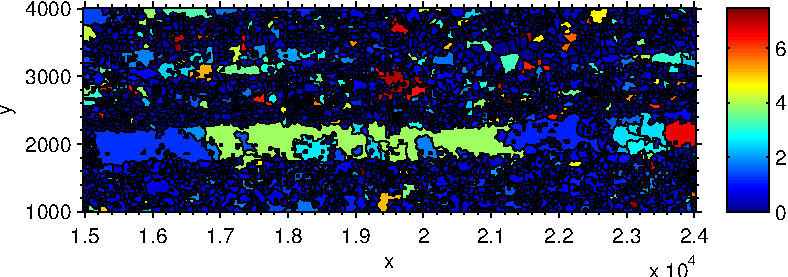
\includegraphics[width=\textwidth]{pic/oriSpread}}
  \end{onlyenv}


  \begin{onlyenv}<4->
    \vspace{-0.3cm}
\begin{lstlisting}[style=input]
grains(oriSpread>5*degree)
\end{lstlisting}
  \end{onlyenv}
  \begin{onlyenv}<4>
\begin{lstlisting}[style=output]
ans = /+Grain2d-Set+/ (show methods, plot)
  file name: mylonite.txt
  grain properties: boundaryEdgeOrder
  EBSD properties: x, y, mis2mean
  Phase Grains Orient.    Mineral Symmetry Crystal reference frame
      1     14      72   Andesina       -1             X||a*, Z||c
      2     17     144     Quartz      -3m      X||a*, Y||b, Z||c*
      3      1       4    Biotite      2/m      X||a*, Y||b*, Z||c
      4     12     138 Orthoclase      2/m      X||a*, Y||b*, Z||c
\end{lstlisting}
  \end{onlyenv}
\end{overlayarea}

\end{frame}

\begin{frame}[fragile]
  \frametitle{Design Principle - Everything is a Vector II }

  \begin{overlayarea}{\textwidth}{\textheight}
\begin{lstlisting}[style=input]
sigma = tensor([[0 0 0];[0 0 0];[0 0 1]],'stress')
\end{lstlisting}
    \begin{onlyenv}<1>
\begin{lstlisting}[style=output]
sigma = stress /+tensor+/ (show methods, plot)
  rank: 2 (3 x 3)

 0 0 0
 0 0 0
 0 0 1
\end{lstlisting}
    \end{onlyenv}
    \begin{onlyenv}<2->
      \vspace{-0.3cm}
\begin{lstlisting}[style=input]
ori = get(grains('Quartz'),'orientation');
\end{lstlisting}
    \end{onlyenv}
    \begin{onlyenv}<2>
\begin{lstlisting}[style=output]
ori = /+orientation+/ (show methods, plot)
  size: 776 x 1
  crystal symmetry: Quartz (-3m, X||a*, Y||b, Z||c*)
  sample symmetry : triclinic
\end{lstlisting}
    \end{onlyenv}
    \vspace{-0.3cm}
    \begin{onlyenv}<3->
\begin{lstlisting}[style=input]
sigmaCS = rotate(sigma,inv(ori))
\end{lstlisting}
    \end{onlyenv}
    \begin{onlyenv}<3>
\begin{lstlisting}[style=output]
sigmaCS = stress /+tensor+/ (show methods, plot)
  size   : 776 x 1
  rank   : 2 (3 x 3)
  mineral: Quartz (-3m, X||a*, Y||b, Z||c*)
\end{lstlisting}
    \end{onlyenv}
    \begin{onlyenv}<4->
      \vspace{-0.3cm}
    \begin{lstlisting}[style=input]
m = Miller(0,0,0,1,symmetry('quartz'))
n = Miller(1,1,-2,0,symmetry('quartz'))
tauMax = calcShearStress(sigmaCS,m,n,'symmetrise')
\end{lstlisting}
    \end{onlyenv}


    \begin{onlyenv}<5->
      \vspace{-0.3cm}
\begin{lstlisting}[style=input]
plot(grains('quartz'),'property',tauMax')
\end{lstlisting}
      \centerline{
      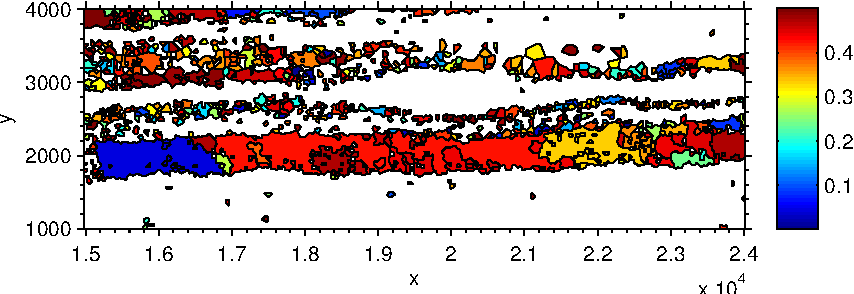
\includegraphics[width=\textwidth]{pic/tau}}
    \end{onlyenv}

  \end{overlayarea}






\end{frame}


% \begin{frame}
%   \frametitle{Do everything in parallel}
% \end{frame}

\end{document}


%%% Local Variables:
%%% mode: latex
%%% TeX-master: t
%%% End:
